% !TeX encoding = UTF-8
% !TeX program = xelatex
% !TeX spellcheck = en_US

\documentclass{npr}
\usepackage{amsmath}
\usepackage{booktabs}
\usepackage{graphicx}
\usepackage{siunitx}
\usepackage{afterpage}
\classsetup{
  % 配置里面不要出现空行
  title  = {$^{18}\mathrm{O}$+$^{152}\mathrm{Sm}$近垒及垒下光学势研究},
  title* = {Study of the Optical Potential for $^{18}\mathrm{O}$+$^{152}\mathrm{Sm}$ at Near- and Sub-barrier Energies},
  authors = {
    luhao = {
      name         = {卢灏},
      name*        = {LU Hao},
      affiliations = {ciae},
      % 只需要第一作者提供个人简介
      biography    = {卢灏(2000--)，男，硕士研究生},
      % 第一作者和通讯作者需要提供电子邮件
      email        = {luhao@ciae.ac.cn},
      % 通讯作者
      corresponding = false,
    },
    linchengjian = {
      name         = {林承键$^\dagger$},
      name*        = {LIN Chengjian$^\dagger$},
      affiliations = {ciae,gx},
      email        = {cjlin@ciae.ac.cn},
      corresponding = true
    },
    yanglei = {
      name         = {杨磊$^\dagger$},
      name*        = {YANG Lei$^\dagger$},
      affiliations = {ciae},
      email        = {yang_lei@ciae.ac.cn},
    },
    mananru = {
      name         = { 马南茹 },
      name*        = {MA Nanru},
      affiliations = {ciae},
      email        = {mnr209@163.com},
    },
        jiahuiming = {
      name         = { 贾会明 },
      name*        = {JIA Huiming},
      affiliations = {ciae},
      email        = {jiahm@ciae.ac.cn},
    },
        wenpeiwei = {
      name         = { 温培威 },
      name*        = {WEN Peiwei},
      affiliations = {ciae},
      email        = {wenpeiwei@hotmail.com},
    },
        yangfeng = {
      name         = { 杨峰 },
      name*        = {YANG Feng},
      affiliations = {ciae},
      email        = {martin@ciae.ac.cn},
    },
        luotianpeng = {
      name         = { 骆天鹏 },
      name*        = {LUO Tianpeng},
      affiliations = {ciae},
      email        = {tpluo_ciae@163.com},
    },
        changchang = {
      name         = { 常昶 },
      name*        = {CHANG Chang},
      affiliations = {ciae},
      email        = {changchangCCC@outlook.com},
    },
        yincheng = {
      name         = { 尹诚 },
      name*        = {YIN Cheng},
      affiliations = {ciae},
      email        = {244624698@qq.com},
    },
        huangzhijie = {
      name         = { 黄志杰 },
      name*        = {HUANG Zhijie},
      affiliations = {ciae},
      email        = {3197429869@qq.com},
    },
        gufuchang = {
      name         = { 顾富昌 },
      name*        = {GU Fuchang},
      affiliations = {zhongshan},
      email        = {gufch3@mail2.sysu.edu.cn},
    },
        wanghaorui = {
      name         = { 王浩睿 },
      name*        = {WANG Haorui},
      affiliations = {ciae},
      email        = {bg8335@126.com},
    },
    moshaowen = {
      name         = { 莫绍文 },
      name*        = {MO Shaowen},
      affiliations = {ciae},
      email        = {1181337963@qq.com},
    },
    wuchenxu = {
      name         = { 武晨旭 },
      name*        = {WU Chenxu},
      affiliations = {ciae},
      email        = {wucx@ciae.ac.cn},
    },
    fulingyi = {
      name         = { 傅凌逸 },
      name*        = {FU Lingyi},
      affiliations = {ciae},
      email        = {fulinyi523@qq.com},
    },
    lihuiyan = {
      name         = { 李慧艳 },
      name*        = {LI Huiyan},
      affiliations = {ciae},
      email        = {2892853289@qq.com},
    },
        lizhilong = {
      name         = { 李志龙 },
      name*        = {LI Zhilong},
      affiliations = {ciae},
      email        = {718575941@qq.com},
    },
        duanhairui = {
      name         = { 段海锐 },
      name*        = {DUAN Hairui},
      affiliations = {ciae},
      email        = {hrduan16@163.com},
    },
        zhusongxian = {
      name         = { 祝颂娴 },
      name*        = {ZHU Songxian},
      affiliations = {ciae},
      email        = {1525547361@qq.com},
    },
        shiyuting = {
      name         = { 侍玉婷 },
      name*        = {SHI Yuting},
      affiliations = {ciae},
      email        = {1134192622@qq.com},
    },
    wanxinxin = {
      name         = { 万欣欣 },
      name*        = {WAN Xinxin},
      affiliations = {ciae},
      email        = {wanxinxin2002@163.com},
    },
  },
  affiliations = {
    ciae = {
      name  = {中国原子能科学研究院，北京　102413},
      name* = {China Institute of Atomic Energy, Beijing 102413, China},
    },
    gx = {
      name = {广西师范大学 物理科学与技术学院，广西核物理与核技术重点实验室，广西 桂林　541004},
      name* = {School of Physical Science and Technology, Guangxi Normal University; Guangxi Key Laboratory of Nuclear Physics and Nuclear Technology, Guilin 541004, Guangxi, China}
    },
    zhongshan = {
      name  = {中山大学中法核工程学院，广东珠海 519082},
      name* = {Sino-French Institute of Nuclear Engineering and Technology, Sun Yat-sen University, Zhuhai 519082, China},
    }
  },
  abstract  = {
    为了研究形变核反应体系光学势随能量变化的关系，本工作首次测量了52-72~MeV六个能量点下$^{18}\mathrm{O}$+$^{152}\mathrm{Sm}$体系的准弹性和弹性散射角分布。弹性散射角分布由高动量分辨的Q3D磁谱仪测量得到，而准弹性散射（包括基态、第一和第二激发态等）角分布由反应靶室内的硅PIN阵列测量得到。在弹性散射角分布中观察到了显著的库仑虹抑制现象，表明该体系存在大形变导致的强库仑激发的耦合，导致弹性散射反应道被吸收而异常地快速下降。
    基于实验角分布数据，采用耦合道 ECIS95 程序提取了各能点下光学势的实部和虚部势深度，获得了其能量依赖行为。结果显示，随着能量降低，光学势虚部出现异常增强，且实、虚部之间不满足色散关系，表现出典型的反常阈异常特征。这一现象首次在形变核体系中被发现，表明除破裂效应外，强库仑激发等强吸收机制同样有可能导致光学势的反常阈行为。
    本研究为探索反常阈异常的起因提供了新的线索。
  },
  abstract* = {
    To investigate the energy dependence of the optical potential in deformed nuclear reaction systems, this work reports the first measurement of quasi-elastic and elastic scattering angular distributions for the $^{18}\mathrm{O}$+$^{152}\mathrm{Sm}$Sm system at six incident energies ranging from 52 to 72 MeV. The elastic scattering angular distributions were measured using the Q3D magnetic spectrometer with high momentum resolution, while the quasi-elastic scattering angular distributions (including the ground state, first and second excited states) were obtained using a silicon detector array inside the reaction chamber. A significant suppression of the Coulomb rainbow was observed in the elastic scattering angular distributions, indicating the presence of strong Coulomb excitation coupling induced by the large deformation of the target nucleus, which leads to an anomalously rapid decrease in the elastic scattering channel due to enhanced absorption.
    Based on the experimental angular distribution data, the real and imaginary parts of the optical potential at each energy point were extracted using the coupled-channels code ECIS95, and their energy-dependent behavior was obtained. The results show that as the incident energy decreases, the imaginary part of the optical potential exhibits an anomalous enhancement, and the real and imaginary parts do not satisfy the dispersion relation, displaying typical characteristics of the anomalous threshold anomaly. This phenomenon is observed for the first time in a deformed nuclear system, indicating that in addition to breakup effects, strong absorption mechanisms such as intense Coulomb excitation can also lead to anomalous threshold behavior in the optical potential.
    This study provides new insights into the origin of the anomalous threshold anomaly.

  },
  keywords  = {光学模型；大形变核；准弹性散射；库仑虹抑制；阈异常; 反常阈异常},
  keywords* = {
    optical model; heavy deformed nuclei; quasi-elastic scattering; Coulomb rainbow suppression; threshold anomaly; abnormal threshold anomaly;
  },
  grants         = {
    国家重点研发计划(批准号: 2023YFA1606402, 2022YFA1602302)；
    国家自然科学基金(批准号: 12235020, 12275360, 12375130)；
    稳定支持基础科研计划。
  },
  % revised-date   = {2014-10-19},
  grants* = {
    National Key Research and Development Program of China (2023YFA1606402, 2022YFA1602302);
    National Natural Science Foundation of China (12235020, 12275360, 12375130);
    Stability Support Program for Basic Scientific Research.
},
  % article-id     = {1007­-4627(2020)\;01-­0040-­03},
  clc            = {O571.1},
  document-code  = {A},
  % doi            = {10.11804/NuclPhysRev.32.03.1},
  % received-date  = {2014-08-10},
  % publish-date   = {2015-01-16},
  volume         = {99},
  number         = {9},
  page           = {1},
}

\newcommand\dif{\mathop{}\!\mathrm{d}}  % 微分符号
\newcommand{\RM}{\ensuremath{\mathrm}}   %正体 既可用于文本模式也可用于数学模式
\newcommand{\me}{\mathrm{e}}  %直立体e
\newcommand{\mi}{\mathrm{i}}  %直立体i
\newcommand{\mj}{\mathrm{j}}  %直立体j
\newcommand{\afrac}[2]{\dfrac{\,#1\,}{\,#2\,}}  %略长分数线
\newcommand{\nn}{\nonumber}  %公式无编号
\newcommand{\nt}{\noindent}
\newcommand{\OO}{~\text{。}}
\newcommand{\PP}{~\text{，}}
\newcommand{\OP}{~\text{；}}
\newcommand{\LT}{\left}
\newcommand{\RT}{\right}

% hyperref 总是在导言区的最后加载
\usepackage{hyperref}



\begin{document}

\maketitle

\section*{引言}
自Fernbach等人\cite{fernbach1949scattering}首次将光学模型应用于描述中子在不同靶核上的核散射与核吸收过程以来，该模型在过去七十年间被广泛采用并取得了巨大成功，现已成为核物理学中最基本的反应模型之一。其核心思想是：入射粒子与靶核相互作用时发生散射或吸收与光学中复折射率介质对光的折射与吸收现象类似\cite{feshbach1958optical,hodgson1971nuclear}。相互作用势即光学势可写为
\begin{equation}
U(r) = V(r) + iW(r),
\end{equation}
其中，实部势 $V(r)$ 描述吸引性的核力作用，决定散射过程中的透射与反射行为；虚部势 $W(r)$ 描述反应通道引起的吸收效应，反映入射通量向准弹性过程的损失。20世纪80年代中期，实验发现光学势在库仑势垒附近具有能量依赖性\cite{baeza1984energy,lilley1985evidence}：当能量降低至库仑势垒以下，虚部势随着非弹性反应道的闭合而急剧减小，从而出现阈值现象；同时实部势在势垒附近呈现出钟罩形的异常增强行为。这一现象由此被称为阈异常\cite{nagarajan1985dispersion,mahaux1986causality,satchler1991heavy,brandan1997interaction}（threshold anomaly，TA）。基于此，光学模型势被表述为
\begin{equation}
U(r;E) = V(r;E) + iW(r;E)
\end{equation}
其中，实部势$V(r;E)$通常可分解为
\begin{equation}
V(r;E) = V_0(r;E) + \Delta V(r;E)
\end{equation}

实部势的第一项源于空间非定域性，通常在大能量范围内呈现缓慢平滑的能量依赖性；第二项称为动力学极化势，由时间非定域性导致，并通过色散关系与虚部势相关联:
\begin{equation}
\Delta V(r;E) = \frac{P}{\pi}\int^\infty_0\frac{W(r;E')}{E'-E}dE'
\label{kk}
\end{equation}
其中P为积分主值。色散关系（一般情况下称为Kramers-Kronig关系）是根据因果律自然得到的结果，描述了介质中的色散效应对波在该介质中传播特性的影响。目前发现大量体系如$^{16}\mathrm{O}$+$^{208}\mathrm{Pb}$\cite{nagarajan1985dispersion}、$^{19}\mathrm{F}$+$^{208}\mathrm{Pb}$\cite{lin2001threshold}、$^{7}\mathrm{Li}$+$^{208}\mathrm{Pb}$\cite{keeley1994optical}、$^{16}\mathrm{O}$+$^{60}\mathrm{Ni}$\cite{fulton1985energy}、$^{32}\mathrm{S}$+$^{40}\mathrm{Ca}$\cite{diaz1989threshold}等，其光学势的实部虚部势深度整体上都满足色散关系，普遍有阈异常的现象。

相较于 $^{16}\mathrm{O}$+$^{208}\mathrm{Pb}$ 这类由球形双幻核组成的紧束缚体系，弱束缚核由于其特殊的结构以及动力学性质，其近垒能区光学势可能呈现出不同的能量依赖行为\cite{hussein2006new,keeley2007fusion}。例如，对于稳定弱束缚核 $^{6}\mathrm{Li}$ 参与的反应体系，如 $^{6}\mathrm{Li}$+$^{28}\mathrm{Si}$\cite{pakou2004elastic}、$^{64}\mathrm{Ni}$\cite{biswas2008study}、$^{80}\mathrm{Se}$\cite{fimiani2012elastic}、$^{138}\mathrm{Ba}$\cite{maciel1999influence}、$^{144}\mathrm{Sm}$\cite{figueira2010energy} 和 $^{208}\mathrm{Pb}$\cite{keeley1994optical}等，实验普遍发现光学势虚部在入射能量降低时反而出现增强。Hussein等人将这种情况称为“破裂阈异常”（Breakup threshold anomaly，BTA）\cite{hussein2006new}，认为这类体系不满足色散关系的原因可能是体系易于破裂，导致入射道通量向连续态通道的大量流失，从而使光学势虚部在势垒附近呈现出异常增强的趋势。同样，对于弱束缚核体系$^{9}\mathrm{Be}$+$^{208}\mathrm{Pb}$、$^{209}\mathrm{Bi}$
\cite{gomez2015energy}，光学势也表示出了明显的破裂阈异常行为。但是，对于与$^{6}\mathrm{Li}$+$^{208}\mathrm{Pb}$非常相似的$^{7}\mathrm{Li}$+$^{208}\mathrm{Pb}$体系，其光学势却表现出了与一般情况较为类似的阈异常现象\cite{黄志杰2024近库仑势垒能区}。考虑到$^{7}\mathrm{Li}$（$S_{\alpha}(^7\mathrm{Li})=2.467~MeV$）与$^{6}\mathrm{Li}$（$S_{\alpha}(^6\mathrm{Li})=1.474~MeV$）破裂阈的差异似乎也不足以解释其光学势完全不同的表现，所以在弱束缚核体系上观察到的光学势不满足色散关系的现象也许不应当完全归因于破裂。

此外，在晕核体系如$^{11}\mathrm{Li}$+$^{208}\mathrm{Pb}$\cite{cubero2012halo}、$^{6}\mathrm{He}$+$^{209}\mathrm{Bi}$\cite{yang2014optical}的弹性散射角分布数据中还观察到了强烈的库仑虹抑制，这是破裂连续态强耦合导致入射道通量大量流失的直接表现。同时，$^{6}\mathrm{He}$+$^{209}\mathrm{Bi}$体系的光学势也被发现不满足色散关系。考虑到$^{11}\mathrm{Li}$（$S_{2\mathrm{n}}(^{11}\mathrm{Li})=0.369~MeV$）与$^{6}\mathrm{He}$（$S_{2\mathrm{n}}(^6\mathrm{He})=0.975~MeV$）的破裂阈要比前面的弱束缚核更低，这些体系的破裂阈与库仑虹抑制以及阈异常之间的关系值得更深入的调查。

然而，在大形变核体系也观察到了库仑虹抑制的现象。例如$^{154}\mathrm{Sm}$（$\beta_2$=0.34）或 $^{184}\mathrm{W}$（$\beta_2$=0.25）这样的核具有较大的四极形变参数，其第一激发态能量分别仅为 82~keV 和 110~keV，因此在碰撞过程中极易被激发，非弹激发截面因此显著增大。这种强烈的耦合效应同样会导致入射道通量的大量损失\cite{love1977dynamic}。在 $^{18}\mathrm{O}$+$^{184}\mathrm{W}$ 的弹性散射实验中\cite{thorn1977effect}观察到的库仑虹抑制现象，与在晕核体系中由于破裂连续态强耦合而导致库仑虹被压低的实验现象高度相似\cite{yang2014optical}。

因此，体系光学势的实部与虚部不满足色散关系可能并不仅仅与破裂有关，更普遍的因素应该是强吸收效应（破裂、转移、非弹激发等），因此“反常阈异常”（Abnormal Threshold Anomaly，ATA）可能是对这种现象更通用的描述。通过系统研究大形变核体系光学势随能量变化的行为，一方面可以有助于确认角分布中的库仑虹抑制现象与光学势中的反常阈异常现象的关联，另一方面可以在弱束缚体系和大形变体系这两类完全不同的体系间一起讨论反常阈异常现象，从而更深入地理解强吸收效应对相互作用势的影响机制，为阐明光学势反常行为提供重要的线索。

目前，与此相关的实验研究仍然十分有限。例如，$^{18}\mathrm{O}$+$^{184}\mathrm{W}$体系的实验仅在单一能点上测量了散射数据\cite{thorn1977effect}；而 $^{16}\mathrm{O}$+$^{152,150,148,144}\mathrm{Sm}$ 体系的实验虽然在多个能量点上测量了弹性散射角分布，但未能从实验数据中可靠地提取光学势参数，从而给出光学势的能量相依性\cite{talon1981coulomb}。这可能与实验统计精度不足、测量能区范围有限、角度覆盖不完整，或相关理论分析方法尚不完善等因素有关。因此，大形变核体系光学势的能量依赖特性仍有待进一步深入研究。

本工作选取形变核 $^{152}\mathrm{Sm}$ 为靶核，其四极和八极形变参数分别为 $\beta_2 = 0.308$、$\beta_4 = 0.127$，基态为$0^+$态，第一、二激发态（$2^+$ 和 $4^+$）的激发能分别为 121~keV 和 366~keV\cite{nudat}。与 $^{154}\mathrm{Sm}$ 第一激发态的激发能（82~keV）相比，$^{152}\mathrm{Sm}$ 的激发能更高，既属于易于激发的大形变核，又避免因激发能过小对探测器分辨能力提出过高要求。

实验方面，在近库仑势垒能区测量了 $^{18}\mathrm{O}+^{152}\mathrm{Sm}$ 体系的弹性和准弹性散射角分布，并利用 ECIS95 程序对实验数据进行光学模型拟合，提取了该体系的光学势参数。进一步通过分析光学势实部和虚部的能量依赖关系，探讨了色散关系在大形变核体系中的适用性。



\section{实验设置}
本实验在中国原子能科学研究院的 HI-13 串列加速器 Q3D 磁谱仪终端上开展。
实验设施整体情况如图\ref{装置}。
\begin{figure}[h]
\centering
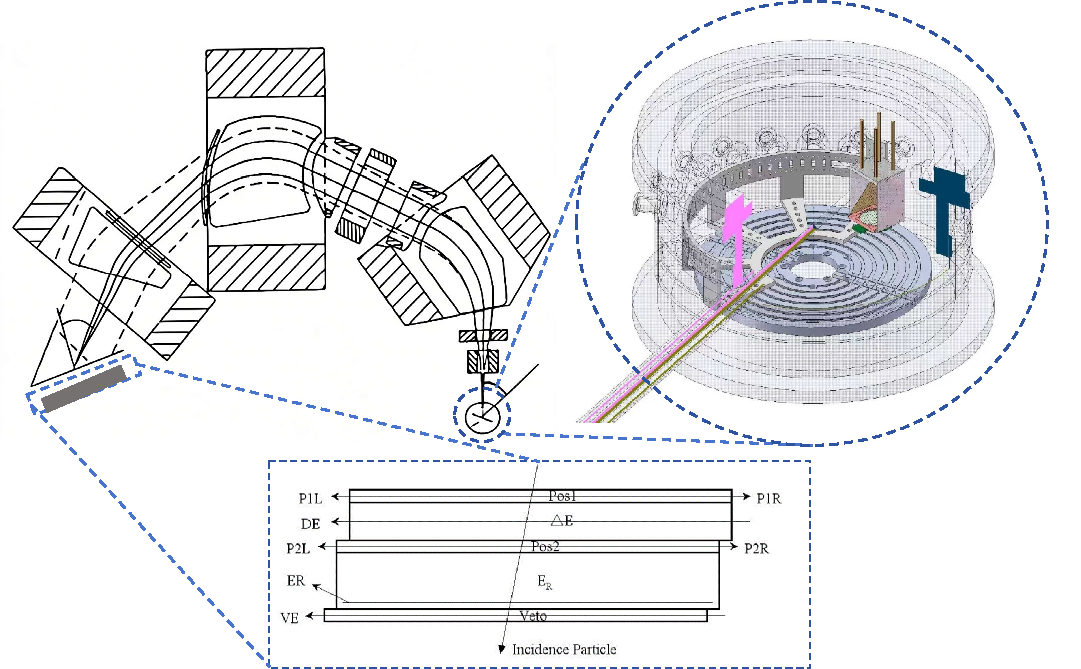
\includegraphics[width=0.95\linewidth]{images/装置.pdf}
\caption{实验设施示意图}
\label{装置}
\small 左上方为Q3D磁谱仪示意图，右上方为反应靶室示意图，下方为焦面探测器示意图。
\end{figure}

使用$^{18}\mathrm{O}$ 束流（流强约20~$e$nA）轰击厚度约 10~$\mathrm{\mu} \mathrm{g/cm^2}$ 的$^{152}\mathrm{Sm}$ 靶（碳底衬厚度约  10~$\mathrm{\mu} \mathrm{g/cm^2}$），能量分别为 72、68、64、60、56 和52~MeV（相应于0.79$V_\mathrm{B}$～1.09$V_\mathrm{B}$，$V_\mathrm{B} \approx 66$~MeV\cite{wen2022new}）。在反应靶室中从25°-160°水平放置28块硅PIN探测器用于测量准弹性角分布；在25°放置3块硅PIN探测器用于束流监视器，测量卢瑟福散射。束流在反应靶室轰击靶后可以进入Q3D磁谱仪，经过磁谱仪偏转后进入焦面靶室。在焦面靶室放置一块五层的焦面探测器用于测量弹性散射角分布，其有效探测长度为50~cm，充入80~torr的CF4气体，并为每一层的一端加上了1000~V的高压。Q3D磁谱仪可以在-20～140°的范围进行旋转。


\section{结果分析和讨论}%3


\subsection{$^{18}$O+$^{152}$Sm的准弹角分布}%3.1


% 根据硅阵列数据得到的准弹性散射角分布
在实验中，PIN探测器的能量分辨约0.4~MeV，无法直接区分出弹性散射反应道与准弹性散射反应道对应的峰。因此，能量谱主峰中至少包含了$^{152}\mathrm{Sm}(^{18}\mathrm{O},^{18}\mathrm{O})^{152}\mathrm{Sm}_{0^+}$、$^{152}\mathrm{Sm}(^{18}\mathrm{O},^{18}\mathrm{O})^{152}\mathrm{Sm}_{2^+}$、$^{152}\mathrm{Sm}(^{18}\mathrm{O},^{18}\mathrm{O})\mathrm{Sm}_{4^+}$反应道的计数。另外，实验中为了让靶始终面向Q3D磁谱仪的入口，需要不断旋转靶角，导致总有一些角度的硅探测器与靶框形成较大的角度，并使得谱中显示出大幅度的低能拖尾。
因此，对谱中主峰进行了拖尾高斯拟合，以期望尽可能在各轮数据间一致地得到峰计数，拖尾高斯函数表达式为：

\begin{multline}
f(x; A, t, u, c) = \frac{A}{2t} \, \exp\!\left( \frac{x-u}{t} + \frac{c^2}{2t^2} \right) \cdot \\
 \operatorname{erfc}\!\left( \frac{1}{\sqrt{2}} \left( \frac{x-u}{c} + \frac{c}{t} \right) \right)
\end{multline}
其中$\mu$、c与标准高斯函数的均值、标准差相对应，函数经过设计使得A恰好为函数的积分，t则对应函数拖尾的程度。
图\ref{pin}为$E_\mathrm{lab} = 72$~MeV下由位于45°的硅探测器得到的能量谱。

\begin{figure}[h]
\centering
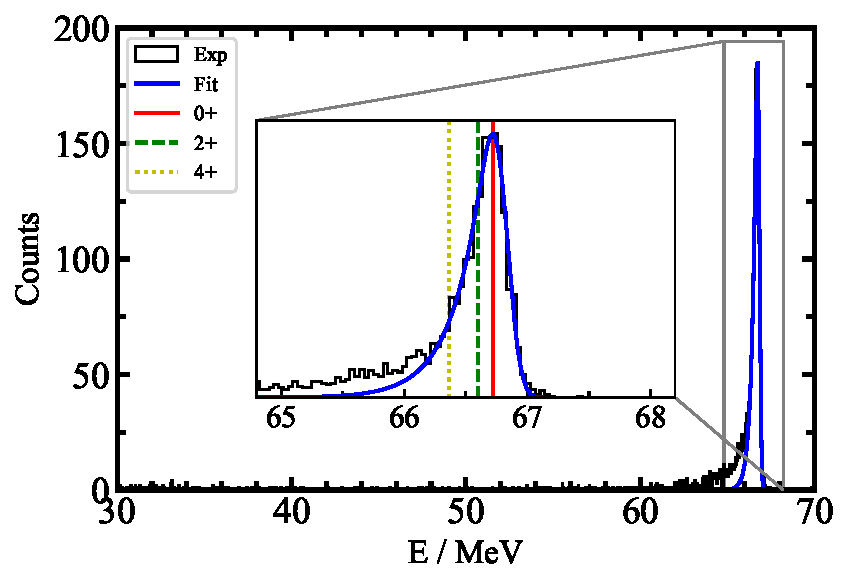
\includegraphics[width=1\linewidth]{images/pin_with_inset.pdf}
\caption{典型的pin探测器能量谱}
\small 阶梯线段为实验数据，曲线表示拖尾高斯的拟合结果，详情图中从高能到低能的三条竖线分别表示$0^+$、$2^+$、$4^+$三个反应道出射粒子总能量对应的峰位。PIN探测器的能量分辨无法直接区分出三个反应道对应的峰，对应计数用于准弹性散射角分布。
\label{pin}
\end{figure}
最终结果在图\ref{result}中使用矩形点表示，误差仅考虑统计误差。尽管这种数据处理方法可以应对探测器与靶框角度过大的问题，但也可能将额外的反应道计数加入到准弹性散射的总计数中，这为基于硅阵列数据得到的角分布带来了一些误差。这些误差在垒下的能点较为明显，体现为相对截面的值存在一些涨落。

\subsection{$^{18}$O+$^{152}$Sm的弹性散射角分布}

\begin{figure*}
\centering
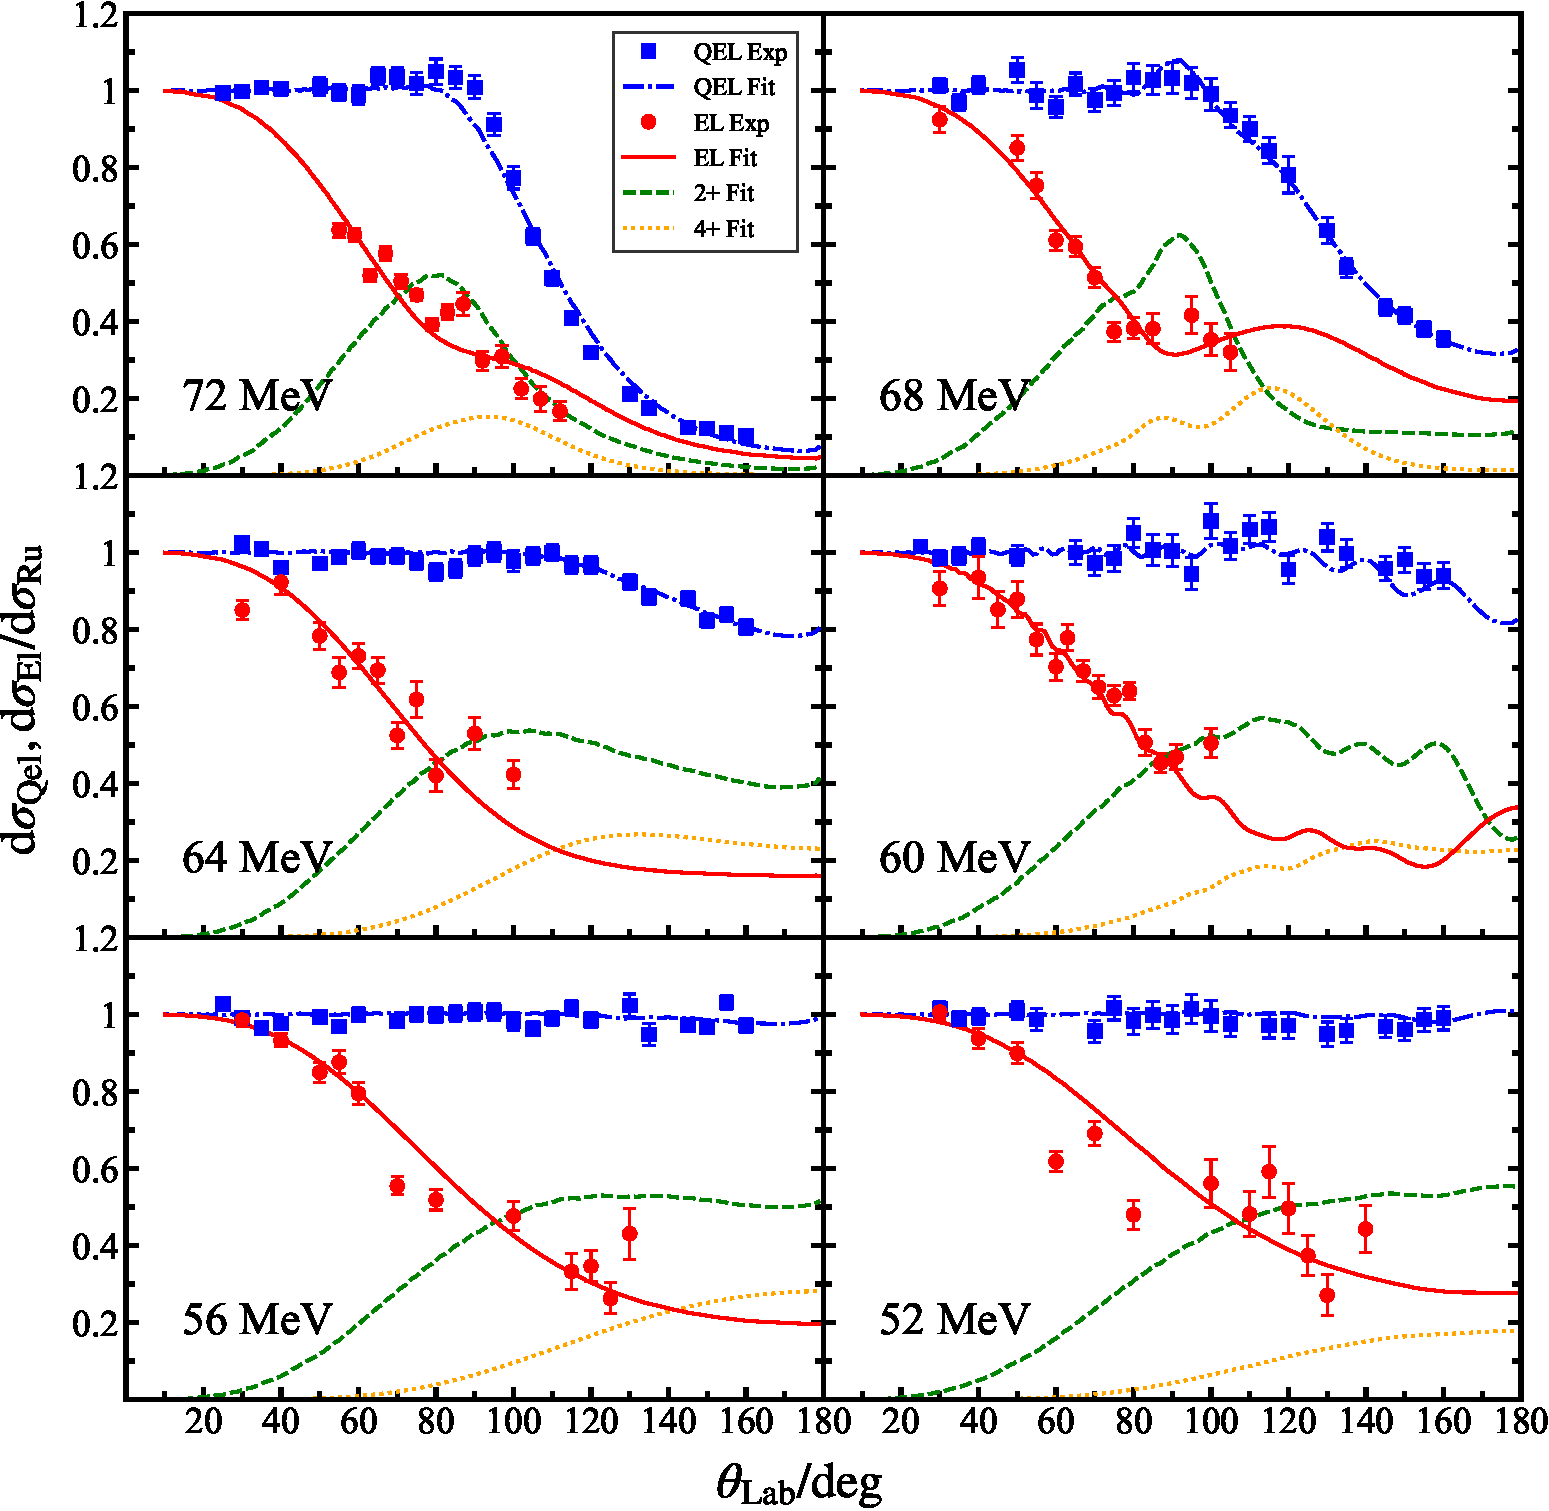
\includegraphics[width=0.8\linewidth]{images/result.pdf}
\caption{各个能量下实验和预测的准弹性散射以及弹性散射截面}
\small 图中矩形为实验准弹性散射角分布，圆形为实验弹性散射角分布，曲线中点划线表示模型预测的准弹性散射角分布，实线表示预测的弹性散射角分布，虚线表示预测的$4^+$反应道截面的角分布，点线表示预测的$2^+$反应道截面的角分布
\label{result}
\end{figure*}
% }
使用Q3D磁谱仪搭配焦面探测器的探测体系对弹核质量、探测器摆放位置等实验细节因素非常敏感。本次实验缺乏有效的调试工具以及充分的束流时间，导致未能获得最理想的分辨。图\ref{focal}为$E_\mathrm{lab} = 60$~MeV下，Q3D角度为66°时，焦面探测器得到的位置谱。由图可见，最终的分辨无法将$^{152}\mathrm{Sm}(^{18}\mathrm{O},^{18}\mathrm{O})$ $^{152}\mathrm{Sm}_{0^+}$与$^{152}\mathrm{Sm}(^{18}\mathrm{O},^{18}\mathrm{O})^{152}\mathrm{Sm}_{2^+}$两个反应道对应的峰直接分开，因此需要通过多高斯拟合来得到各个反应道的计数。

拟合的函数可以表示为：
\begin{multline}
f(x) = G(x,A_{\mathrm{0^+}},\mu_{\mathrm{0^+}},\sigma_{\mathrm{0^+}}) + G(x,A_{2^+},\mu_{2^+},\sigma_{2^+}) \\
+ G(x,A_{4^+},\mu_{4^+},\sigma_{4^+})
\end{multline}
其中
$$
G(x,A,\mu,\sigma) = A e^{-\frac{(x-\mu)^2}{2\sigma^2}}
$$
为标准高斯函数，而$x$则为焦面探测器的位置，$f(x)$为一个合适的分bin下$x$位置对应的计数。

这里同时对三个反应道进行高斯拟合，一共需要得到9个参数。由于$^{152}\mathrm{Sm}$三个态的能量展宽都很小，因此假定三个峰的展宽相同，也就是
$$
\sigma_{\mathrm{0^+}} = \sigma_{2^+} = \sigma_{4^+}
$$
另外，因为已知三个反应道的能量差，在动量刻度后就可以确定三个峰之间的位置差，于是最终只需要拟合5个参数：$\mu_{\mathrm{0^+}},\sigma_{\mathrm{0^+}},A_{\mathrm{0^+}},A_{2^+},A_{4^+}$。拟合得到的各个高斯函数用曲线绘制在图\ref{focal}中。

\begin{figure}[h]
\centering
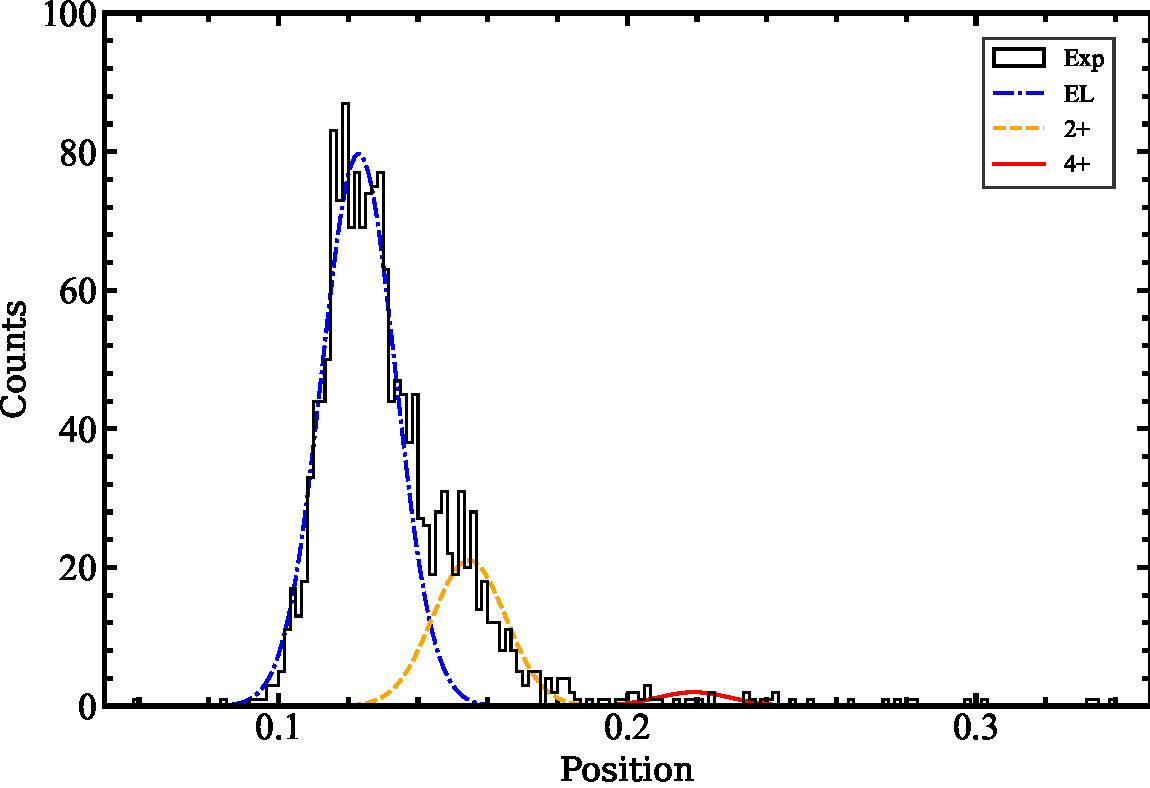
\includegraphics[width=1\linewidth]{images/focal.pdf}
\caption{焦面探测器位置谱}
\small 负方向为高能端，正方向为低能端，阶梯线段为实验数据，从高能到低能端的三条曲线表示多高斯拟合$0^+$、$2^+$、$4^+$三个反应道的结果。
\label{focal}
\end{figure}
最终得到的弹性散射角分布在图\ref{result}中使用圆形点表示，误差仅考虑统计误差。从$^{152}\mathrm{Sm}(^{18}\mathrm{O},^{18}\mathrm{O}_{\mathrm{0^+}})$反应的弹性散射角分布数据中，可以观察到很强的库仑虹抑制。这一现象与大形变体系$^{16}\mathrm{O}+^{152}\mathrm{Sm}$\cite{kim1979nuclear,talon1981coulomb}、$^{18}\mathrm{O}+^{184}\mathrm{W}$\cite{thorn1977effect}中的观测结果一致。
% 这里可以加几个例子


\subsection{光学势和色散关系}%3.3
使用光学模型对准弹性散射和弹性散射的实验数据进行同时拟合，可以得到每一个能量下的光学势参数。使用的光学模型的相互作用势$U(r)$可以表示为：
\begin{equation}
U(r)= V_C(r) - V_0f(r,R_V,a_V) - iW_0f(r,R_W,a_W)
\label{opt}
\end{equation}
其中，$V_C$为弹核与靶核之间的库仑势，一般可以用一个特定半径的电荷均匀分布的库仑场来表示：
\begin{equation}
V_C(r) = 
\begin{cases} 
\dfrac{(3R_C^2 - r^2) Z_P Z_T e^2}{2R_C^3}, & r < R_C \\[1em]
\dfrac{Z_P Z_T e^2}{r}, & r \geq R_C 
\end{cases}
\end{equation}
其中半径$R_C=r_C(A_T^{1/3}+A_P^{1/3})$，$r_C$为约化库仑半径，$A_T,A_P,Z_T,Z_P$分别为靶核和弹核的质量数和电荷数。

而光学势中的$V_0f(r,R_V,a_V)$和$iW_0f(r,R_W,a_W)$即为实部和虚部势，都通常分成深度和形状因子两个部分。$V_0$和$W_0$分别为实部和虚部的势深度，$f$则为实部和虚部的形状因子，一般可以采用Woods-Saxon势的形式：
\begin{equation}
f(r, R_i, a_i) = \left[ 1 + \exp\left(\frac{r - R_i}{a_i}\right) \right]^{-1}
\end{equation}

\begin{equation}
R_i = r_i(A_P^{1/3} + A_T^{1/3}) \quad i = V, W
\end{equation}
于是，这个光学势一共有6个待定参数，分别为实部的$V_0$、$r_V$、$a_V$和虚部的$W_0$、$r_W$和$a_W$。

在实际拟合中，使用的约化库仑半径$r_C=1.25$~fm\cite{kim1979nuclear}，以及在两个不同来源中一致的形状因子参数：$r_V=2.02~fm$，$r_W=2.06~fm$，$a_V=0.5~fm$，$a_W=0.55~fm$\cite{kim1979nuclear,talon1981coulomb}。每个能点只需要对两个势深度参数进行拟合。

使用ECIS95程序对实验准弹性散射和弹性散射角分布数据进行双参数拟合\cite{raynal1994ecis}，得到了每个能点的实部$V_0$和虚部的势深度$W_0$。其中，在ECIS的输入文件中使用了$\beta_2 = 0.308$，$\beta_4 = 0.127$作为四极形变参数和八极形变参数，考虑了对称转动耦合。

% \begin{figure}
% \centering
% \includegraphics[width=1\linewidth]{images/72.pdf}
% \caption{拟合结果与参考文献的对比}
% \small 图中方形为实验准弹性散射角分布，圆形为实验弹性散射角分布，实线表示本工作模型预测的结果，虚线表示Talon等的结果，点划线表示Kim的结果，点线表示Zhao等的结果。
% \label{72}
% \end{figure}

将拟合得到的参数重新代入表达式~\eqref{opt}中，可以得到模型预测的各个反应道的反应截面，在图\ref{result}中用曲线表示。
从图中可以看到，模型一定程度上重现了准弹性散射的实验数据，但是对弹性散射实验数据的拟合误差较大，这主要受限于弹性散射实验数据本身的误差和涨落。但是如果仅使用准弹性散射数据对光学模型参数进行拟合，失去弹性散射数据约束后的模型结果不确定性会大幅增加，特别是在垒下能点无法得到有意义的实部虚部势深度。这是因为当体系能量低于库仑势垒，相互作用过程由库仑力主导，核力的影响有限。从图中不同能量下准弹性散射角分布的变化趋势可以看到，随着能量从高到低，角分布开始偏离卢瑟福散射（即 d$\sigma / $d$\sigma_{Ru} < 1$）的特征角度逐渐向大角度方向移动；当能量低于库仑势垒后，截面与卢瑟福散射的比值维持在一附近，基本上都是卢瑟福散射。并且随着能量降低，核力的影响也逐渐减小，由库仑散射与核散射相干叠加引起的明暗条纹和库仑虹也变得微弱直至不可见。因此，垒下的准弹性散射数据对核势（尤其是实部）的敏感度极低，几乎不包含可以约束光学势深度的有效信息。这使得模型的可靠拟合高度依赖于弹性散射数据的约束。目前拟合结果与实验数据的整体趋势较为一致，当然在精度方面还有一些提升空间。

从$^{152}\mathrm{Sm}(^{18}\mathrm{O},^{18}\mathrm{O})^{152}\mathrm{Sm}_{2^+}$、$^{152}\mathrm{Sm}(^{18}\mathrm{O},^{18}\mathrm{O})^{152}\mathrm{Sm}_{4^+}$两个反应道角分布的拟合结果来看，模型认为在库仑激发的相对截面总是在前角随着角度增大而快速上升，这与库仑虹抑制、弹性散射相对截面的快速下降相对应，表示入射道通量就是从弹性散射流失到了库仑激发的反应道上。而随着能量降低，背角的库仑激发相对截面在逐渐上升，表示能量越低，在背角库仑激发占比就越大。这可能也是因为核力的影响随着能量降低逐渐减小，库仑力逐渐占主导的结果。
% 由图\ref{72}对于72~MeV能点，拟合得到的光学势参数所给出的弹散、非弹激发曲线的趋势与$^{16}\mathrm{O}+^{152}\mathrm{Sm}$\cite{talon1981coulomb,kim1979nuclear}、$^{12}\mathrm{C}+^{152}\mathrm{Sm}$\cite{zhao1994comparison}体系中的情况基本一致————随着角度增加，弹性散射的通道被快速吸收，2+态对应的反应道截面在70-80°达到最大，而4+态则是在80-95°达到最大。这显示出以$^{152}\mathrm{Sm}$为靶核这样的大形变体系的截面变化的共同趋势。


根据拟合结果，给出了$^{18}\mathrm{O}+^{152}\mathrm{Sm}$体系在六个能点下光学势的能量相依性，如图\ref{final}所示，详细数据见表\ref{excel}。误差由卡方最小化得到的协方差矩阵的对角元计算得出。
\begin{table}[htbp]
\centering
\begin{tabular}{ccccc}
\toprule
Energy (MeV) & V (MeV) & W (MeV) & $\chi^2_{\text{Qel}}$/pt & $\chi^2_{\text{El}}$/pt \\

\midrule   

72 & 7.14 \pm 0.46 & 2.12 \pm 1.22 & 3.08 & 8.70 \\
68 & 11.09 \pm 3.55 & 0.86 \pm 1.84 & 0.63 & 2.34 \\
64 & 6.94 \pm 1.27 & 1.17 \pm 0.80 & 1.09 & 7.32 \\
60 & 25.50 \pm 4.01 & 0.66 \pm 1.03 & 1.27 & 3.23 \\
56 & 1.51 \pm 4.90 & 3.47 \pm 3.63 & 1.54 & 4.78 \\
52 & 2.47 \pm 8.32 & 7.25 \pm 4.94 & 0.59 & 7.34 \\
\bottomrule
\end{tabular}
\caption{ECIS95程序拟合得到的光学势参数及其拟合优度}
\label{excel}
\end{table}


图中实验得到的实部势深度在库仑势垒($\approx$60~MeV)附近有一个明显的凸起，这与典型的阈异常现象相似。由于能点有限并且间隔较大，还无法对实部行为给出更详细的描述。但是虚部势深度随着能量降低却反常地有抬升的趋势，这与$^{6}\mathrm{Li}+^{208}\mathrm{Pb}$体系的光学势十分相似\cite{keeley1994optical}。为了通过虚部得到实部的预测曲线，首先要对虚部进行分段线性拟合。普通的阈异常体系可以使用一个在反应阈值开始，虚部从0开始上升到一个平台的线性模型，表达式如下：
\begin{equation}
W(E) = 
\begin{cases}
0, & E \le E_a \\[1ex]
W_{0s} \, \dfrac{E - E_a}{E_b - E_a}, & E_a < E < E_b \\[1ex]
W_{0s}, & E \ge E_b
\end{cases}
\end{equation}
而实验得到的虚部势随着能量降低而抬升，这无法指示出一个反应阈值，也无法应用这样简单的线性模型。因此，此处使用一个虚部由初值下降到平台的线性模型进行拟合，表达式如下：
\begin{equation}
W(E) = 
\begin{cases}
W_{0s}, & E \le E_a \\[1ex]
W_{0s} - (W_{0s} - W_{1s}) \, \dfrac{E - E_a}{E_b - E_a}, & E_a < E < E_b \\[1ex]
W_{1s}, & E \ge E_b
\end{cases}
\end{equation}
当然，该模型仅作为一种经验性的参数化方式，用于定性检验色散关系的预期行为。
得到虚部的模型后，再通过式~\eqref{kk}计算得到了根据色散关系预测的实部理论曲线。理论曲线预测实部势深度将会在56~MeV附近达到极小值，并在60~MeV附近有一个拐点；但是实验的实部势深度是在60~MeV附近达到了极大值，拐点的位置则可能在60-64~MeV之间，实验的结果显著偏离了色散关系的预测。基于目前的数据所给出的结论是，该体系的光学势并不满足色散关系，表现出反常阈异常的特征。

值得强调的是，对于垒下的两个能点52、56~MeV，拟合得到的光学势参数误差很大。这是因为当前光学势的拟合中仅对两个势深度参数进行拟合，数据的误差会直接导致参数值的偏离。此外，尽管研究中使用的光学势形状因子参数可以一定程度地重现实验数据，但是这并不代表目前使用的就是最佳的参数，考虑到从弹性散射与准弹性散射实验数据抽取光学势参数存在Igo模糊的问题\cite{lin2015}，这可能也会加大结果的不确定性。
因此，只有基于更丰富、更精确的实验数据，并在拟合过程中更全面地考虑各参数之间的相互影响，才能得到该体系光学势行为的更有力的结论。
\begin{figure}
\centering
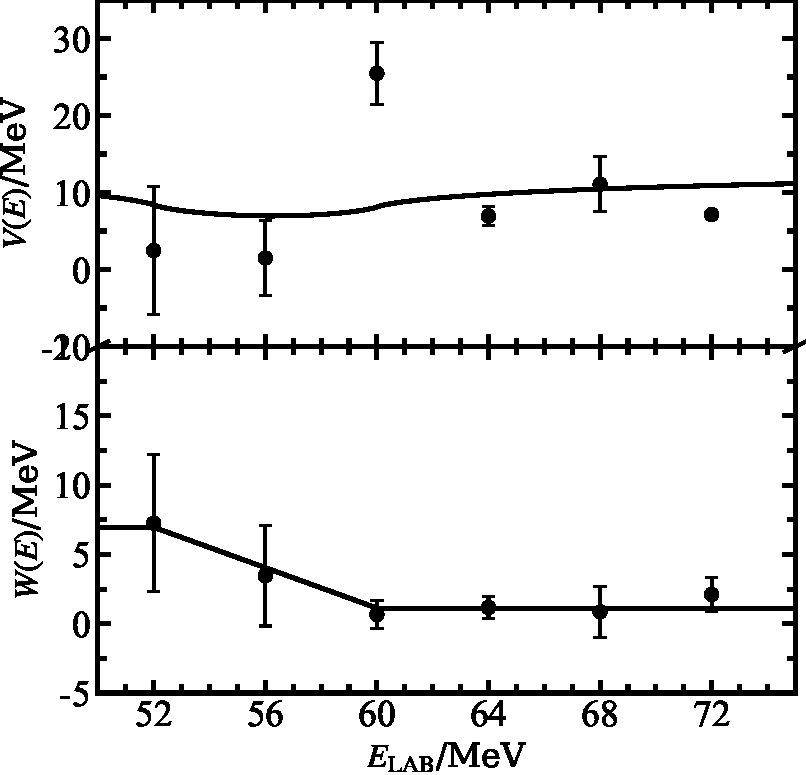
\includegraphics[width=1\linewidth]{images/final.pdf}
\caption{光学势的能量相依性}
\small 图中上半部分表示实部势深度，下半部分表示虚部势深度。原点表示实验值。虚部的拟合结果用线段表示，由虚部及色散关系得到的实部预测值用曲线表示。
\label{final}
\end{figure}

\section{小结}%4

在实验室能量为72, 68, 64, 60, 56, 52~MeV共六个能点下，首次测量了$^{18}\mathrm{O}+^{152}\mathrm{Sm}$体系的准弹性散射角分布以及弹性散射角分布。其中，准弹性散射角分布至少包含了$^{152}\mathrm{Sm}(^{18}\mathrm{O},^{18}\mathrm{O})^{152}\mathrm{Sm}_{0^+}$、$^{152}\mathrm{Sm}(^{18}\mathrm{O},^{18}\mathrm{O})^{152}\mathrm{Sm}_{2^+}$、$^{152}\mathrm{Sm}(^{18}\mathrm{O},^{18}\mathrm{O})^{152}\mathrm{Sm}_{4^+}$三个反应道，而弹性散射角分布在各个角度的计数是通过多高斯函数在分辨不足的谱中拟合得到的。弹性散射角分布的结果中观察到了明显的库仑虹抑制，这个结果表明，在$^{18}\mathrm{O}+^{152}\mathrm{Sm}$的反应体系中存在大形变导致的强库仑激发的耦合，导致弹性散射反应道被吸收而异常地快速下降。

基于准弹性散射和弹性散射的实验数据，进行了光学模型参数的拟合，提取出各个能点下光学势的实部和虚部的势深度。这也是首次在大形变体系中得到了光学势的能量相依性。结果表明，体系的实部和虚部之间的行为不符合色散关系，还出现了随着能量降低而虚部抬升的行为，这是首次在破裂反应体系之外观察到了反常阈异常的现象。破裂和库仑激发这两种截然不同的反应机制都能与反常阈异常的现象相联系，并且两个体系光学势的变化趋势也有相似性。这些结果与强吸收会影响色散关系成立的猜测一致。考虑到角分布与光学势的联系非常直接，也可以猜测类似观察到角分布抑制的体系，例如$^{11}\mathrm{Li}+^{208}\mathrm{Pb}$或者是$^{16}\mathrm{O}+^{184}\mathrm{W}$的体系也会在光学势的能量相依性上表现出反常阈异常的现象。

值得指出的是，本次实验的能点较少，并且数据的精度还未达到最理想的情况，需要进行更系统、更高精度的实验，才能更完整地描述体系的光学势的行为。这些工作可以对大形变体系的光学势研究提供参考。



\bibliographystyle{npr}
% \bibliographystyle{plain}
\bibliography{18O152Sm}



\maketitle


\end{document}
